\section{Cinemática} \label{sec:cinematica}

La cinemática es la ciencia del movimiento que estudia el movimiento sin considerar las fuerzas que lo causan. Dentro de la ciencia de la cinemática, se analizan la posición, la velocidad, la aceleración y todas las derivadas de orden superior de las variables de posición a partir de las variables articulares del sistema para analizar el comportamiento de los eslabones y articulaciones de un manipulador.
	\begin{figure}[H]
	\centering
	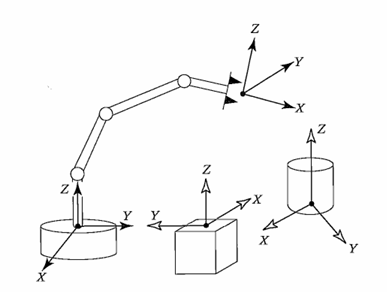
\includegraphics[width=0.7\textwidth]{img/Cinematica.png}
	\caption{Se asignan sistemas de coordenadas o 'marcos de referencia' al manipulador y a los objetos en el entorno.}
	\label{fig:Cinematica}
\end{figure}
Los manipuladores están formados por eslabones rígidos conectados mediante articulaciones que permiten el movimiento relativo entre ellos. Estas articulaciones cuentan con sensores de posición para medir dicho movimiento. En articulaciones rotatorias se habla de ángulos articulares, y en las deslizantes (prismáticas), de desplazamiento lineal o offset.

El número de grados de libertad de un manipulador indica cuántas variables independientes se necesitan para definir su posición completa. En manipuladores industriales típicos, cada articulación representa un grado de libertad, ya que son cadenas cinemáticas abiertas con articulaciones controladas individualmente.

En el extremo del manipulador se encuentra el efector final, que puede ser una herramienta específica como una pinza o un soplete. Para describir la posición del manipulador, se define un marco de coordenadas (tool frame) en el efector y otro en la base fija (base frame), y se analiza la relación entre ambos.


Para el proceso sobre cómo se llevó a cabo el algoritmo en Matlab, ir a la  \hyperref[sec:proceso_cinematica]{sección del proceso de Cinemática}.

\subsection{Cinemática Directa}

La \textbf{cinemática directa} consiste en determinar la posición y orientación del efector final del robot con base en los valores conocidos de las variables articulares. Este es el \textit{problema geométrico estático} de calcular la posición y orientación del efector final del manipulador. Específicamente, dado un conjunto de ángulos articulares, el problema de la cinemática directa consiste en calcular la posición y orientación del marco de la herramienta (\textit{tool frame}) con respecto al marco base (\textit{base frame}). A veces, se considera este proceso como un \textit{cambio de representación} de la posición del manipulador, pasando de una descripción en el \textit{espacio articular} a una descripción en el espacio cartesiano.

Para resolver este problema, se utiliza comúnmente el \textbf{método de Denavit-Hartenberg (DH)}, una convención estandarizada que permite representar de forma sistemática la geometría de un manipulador robótico. Este método simplifica el proceso de modelado mediante la asignación de un sistema de coordenadas a cada eslabón del robot y la definición de las transformaciones relativas entre eslabones consecutivos utilizando solo cuatro parámetros:

\begin{itemize}
	\item $\theta$: ángulo de rotación alrededor del eje $z$ (variable para articulaciones rotacionales).
	\item $d$: desplazamiento a lo largo del eje $z$ (variable para articulaciones prismáticas).
	\item $a$: longitud del eslabón, medida a lo largo del eje $x$.
	\item $\alpha$: ángulo de torsión, es decir, la rotación alrededor del eje $x$ entre dos ejes $z$ consecutivos.
\end{itemize}

La formulación de Denavit-Hartenberg permite obtener una matriz de transformación homogénea $4 \times 4$ para cada par de eslabones, que incorpora rotaciones y traslaciones en el espacio tridimensional. Al multiplicar secuencialmente estas matrices desde el eslabón base hasta el efector final, se obtiene una única matriz que describe completamente la postura del robot, es decir, la posición y orientación del efector con respecto al sistema de referencia global.

Una de las principales ventajas del método DH es su capacidad para estandarizar el modelado de robots con diferentes configuraciones geométricas, lo que facilita la implementación computacional y la interpretación de resultados. En este proyecto, los parámetros DH fueron determinados a partir del modelo CAD del robot desarrollado en SolidWorks, y posteriormente implementados en \texttt{MATLAB} para calcular las matrices de transformación y verificar los resultados mediante simulación gráfica.

\subsection{Cinemática Diferencial}
La \textbf{cinemática diferencial} se encarga de analizar cómo las velocidades articulares afectan la velocidad lineal y angular del efector final de un manipulador robótico. Este análisis es fundamental para el diseño de sistemas de control y planificación de trayectorias en robótica.

\subsubsection{El Jacobiano}

El \textbf{Jacobiano} es una matriz que relaciona las velocidades articulares del robot con las velocidades lineales y angulares del efector final. Matemáticamente, se expresa como:

\[
\dot{\mathbf{x}} = \mathbf{J}(\mathbf{q}) \, \dot{\mathbf{q}}
\]

donde:
\begin{itemize}
	\item $\dot{\mathbf{x}}$ es el vector de velocidades del efector final (lineales y angulares).
	\item $\mathbf{J}(\mathbf{q})$ es la matriz Jacobiana, que depende de las coordenadas articulares $\mathbf{q}$.
	\item $\dot{\mathbf{q}}$ es el vector de velocidades articulares.
\end{itemize}

Cada columna de la matriz Jacobiana representa la contribución de una articulación individual a la velocidad del efector final. Por ejemplo, en un manipulador con $n$ grados de libertad, la $i$-ésima columna de $\mathbf{J}$ describe el efecto de la velocidad de la articulación $i$ en la velocidad del efector final, considerando que las demás articulaciones están fijas.
	\begin{figure}[H]
	\centering
	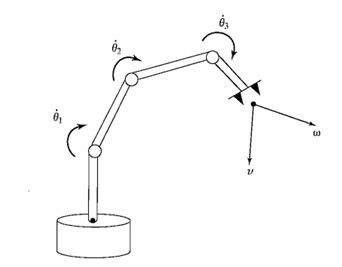
\includegraphics[width=0.7\textwidth]{img/jacobiano.png}
	\caption{La relación geométrica entre las velocidades articulares y la velocidad del efector final puede describirse mediante una matriz llamada Jacobiana.}
	\label{fig:Jacobiano}
\end{figure}

\subsubsection{Aplicaciones del Jacobiano}

El Jacobiano tiene múltiples aplicaciones en robótica, entre las que se incluyen:
\begin{itemize}
	\item \textbf{Análisis de singularidades}: Determinar configuraciones en las que el manipulador pierde grados de libertad o se vuelve incapaz de moverse en ciertas direcciones.
	\item \textbf{Control de velocidad}: Calcular las velocidades articulares necesarias para lograr una velocidad deseada del efector final.
	\item \textbf{Dinámica inversa}: Relacionar fuerzas y torques en el efector final con las fuerzas y torques en las articulaciones.
\end{itemize}

\subsubsection{Cálculo del Jacobiano}

El cálculo de la matriz Jacobiana puede realizarse utilizando métodos analíticos o numéricos. En este proyecto, se empleó el método analítico, derivando las expresiones de las posiciones del efector final con respecto a las coordenadas articulares y calculando las derivadas parciales correspondientes.

\subsubsection{Ejemplo de Jacobiano para una Articulación Rotacional}

Para una articulación rotacional, la contribución a la velocidad lineal del efector final se puede calcular como:

\[
\mathbf{v}_i = \mathbf{z}_{i-1} \times (\mathbf{o}_n - \mathbf{o}_{i-1})
\]

y la contribución a la velocidad angular es:

\[
\boldsymbol{\omega}_i = \mathbf{z}_{i-1}
\]

donde:
\begin{itemize}
	\item $\mathbf{z}_{i-1}$ es el eje de rotación de la articulación $i$ en el marco de referencia base.
	\item $\mathbf{o}_n$ es el vector de posición del efector final.
	\item $\mathbf{o}_{i-1}$ es el vector de posición de la articulación $i$.
\end{itemize}

Estas expresiones se utilizan para construir las columnas correspondientes de la matriz Jacobiana.

\subsubsection{Implementación en MATLAB}

En el presente proyecto, se implementó el cálculo del Jacobiano en \texttt{MATLAB}, utilizando las expresiones analíticas derivadas y verificando los resultados mediante simulaciones. Esta implementación permitió analizar el comportamiento del manipulador en diferentes configuraciones y validar la precisión del modelo cinemático.



\subsection{Cinemática Inversa}

La \textbf{cinemática inversa} es el proceso mediante el cual se determinan los valores articulares necesarios para que el efector final de un robot manipulador alcance una posición y orientación deseadas en el espacio cartesiano tridimensional. En otras palabras, dado un objetivo en términos de coordenadas y orientación en el espacio, el objetivo de la cinemática inversa es encontrar todos los posibles conjuntos de variables articulares que produzcan esa configuración final.

	\begin{figure}[H]
	\centering
	\includegraphics[width=0.7\textwidth]{img/cinematicainv.png}
	\caption{Para una posición y orientación dadas del marco de la herramienta, los valores de las variables articulares pueden calcularse mediante la cinemática inversa.}
	\label{fig:CinematicaInversa}
\end{figure}

Este problema es fundamental en la programación de manipuladores robóticos, ya que las trayectorias y tareas generalmente se especifican en el espacio cartesiano, mientras que el movimiento del robot se controla en su espacio articular. Por lo tanto, es necesario disponer de algoritmos que realicen la conversión entre ambos espacios.

A diferencia de la cinemática directa, las ecuaciones que definen la cinemática inversa son no lineales y, por lo tanto, pueden presentar múltiples soluciones o no tener ninguna, dependiendo de si el punto deseado se encuentra dentro del \textit{espacio de trabajo} del manipulador. Esta complejidad hace que, en muchos casos, no se pueda obtener una solución analítica cerrada, y se deban utilizar métodos numéricos o aproximados.

Uno de los enfoques numéricos más comunes es el uso de algoritmos basados en el \textbf{gradiente del error} y el \textbf{jacobiano}. El jacobiano $\mathbf{J}(\mathbf{q})$ describe la relación entre las velocidades articulares $\dot{\mathbf{q}}$ y las velocidades del efector final $\dot{\mathbf{x}}$ mediante la ecuación:

\[
\dot{\mathbf{x}} = \mathbf{J}(\mathbf{q}) \, \dot{\mathbf{q}}
\]

Este mismo jacobiano se puede utilizar para propagar pequeños cambios en la posición del efector final hacia ajustes en los valores articulares. El \textbf{gradiente del error} entre la posición deseada y la actual se proyecta en el espacio articular mediante el jacobiano transpuesto o su pseudo-inversa, dependiendo del método seleccionado.

Cabe destacar que existen múltiples métodos para resolver el problema de la cinemática inversa, incluyendo:
\subsubsection{Métodos para la Resolución de la Cinemática Inversa}

Existen diversos enfoques para resolver el problema de la cinemática inversa. A continuación, se describen los principales métodos empleados, junto con sus características, ventajas y limitaciones.

\paragraph{1. Métodos Geométricos}

Estos métodos se basan en el análisis de la geometría del robot, utilizando relaciones trigonométricas simples (como la ley de senos y cosenos) para calcular directamente los ángulos articulares.

\begin{itemize}
	\item \textbf{Ventajas:} Rápidos y computacionalmente eficientes. Pueden ofrecer soluciones analíticas cerradas.
	\item \textbf{Limitaciones:} Solo aplicables a robots con geometría sencilla (como robots planos o tipo SCARA).
	\item \textbf{Ejemplo de uso:} Cálculo de ángulos para un manipulador plano de 2 grados de libertad (2-DOF).
\end{itemize}

\paragraph{2. Métodos Algebraicos}

Consisten en plantear y resolver sistemas de ecuaciones no lineales que relacionan las coordenadas del efector final con las variables articulares.

\begin{itemize}
	\item \textbf{Ventajas:} Posibilidad de obtener soluciones exactas si el sistema es resoluble.
	\item \textbf{Limitaciones:} Las ecuaciones pueden ser complejas o no tener solución cerrada, especialmente en manipuladores con múltiples grados de libertad.
	\item \textbf{Ejemplo de uso:} Resolución simbólica de la cinemática inversa de un robot tipo PUMA.
\end{itemize}

\paragraph{3. Métodos Numéricos Iterativos}

Estos métodos aproximan las soluciones mediante iteraciones sucesivas, partiendo de una configuración inicial y ajustando las variables articulares en función del error entre la posición actual y la deseada.

\begin{itemize}
	\item \textbf{Ventajas:} Generalizables a robots complejos. No requieren una solución cerrada.
	\item \textbf{Limitaciones:} Pueden no converger o ser sensibles a la elección del punto inicial.
\end{itemize}

Los principales métodos iterativos son:

\begin{itemize}
	\item \textbf{a) Método del Jacobiano Transpuesto:}
	
	\[
	\Delta \mathbf{q} = \alpha \, \mathbf{J}^T(\mathbf{q}) \, (\mathbf{x}_d - \mathbf{x})
	\]
	
	Utiliza el jacobiano transpuesto para proyectar el error cartesiano al espacio articular. Es simple y efectivo para tareas básicas.
	
	\item \textbf{b) Método de la Pseudo-inversa del Jacobiano:}
	
	\[
	\Delta \mathbf{q} = \mathbf{J}^+(\mathbf{q}) \, (\mathbf{x}_d - \mathbf{x})
	\]
	
	Usa la pseudo-inversa de Moore-Penrose y es adecuado para robots redundantes. Minimiza el error cartesiano de forma más precisa.
	
	\item \textbf{c) Método de Newton-Raphson:}
	
	\[
	\mathbf{q}_{k+1} = \mathbf{q}_k + \mathbf{J}^+(\mathbf{q}_k) \cdot (\mathbf{x}_d - f(\mathbf{q}_k))
	\]
	
	Se basa en una aproximación derivativa para encontrar rápidamente una solución, siempre que se inicie desde una configuración cercana a la correcta.
	
	\item \textbf{d) Método del Gradiente Descendente:}
	
	\[
	E(\mathbf{q}) = \frac{1}{2} \| \mathbf{x}_d - f(\mathbf{q}) \|^2, \quad \mathbf{q}_{k+1} = \mathbf{q}_k - \eta \nabla E(\mathbf{q}_k)
	\]
	
	Minimiza directamente la función de error entre la posición deseada y la alcanzada. Es robusto, pero converge lentamente.
\end{itemize}

\paragraph{4. Comparación de Métodos}

\begin{table}[H]
	\centering
	\begin{tabular}{|l|c|c|c|c|}
		\hline
		\textbf{Método} & \textbf{Precisión} & \textbf{Rapidez} & \textbf{Robustez} & \textbf{Aplicabilidad} \\
		\hline
		Geométrico & Alta & Alta & Media & Robots simples \\
		Algebraico & Alta & Media & Media & Robots con solución cerrada \\
		Jacobiano Transpuesto & Media & Alta & Media & Robots generales \\
		Pseudo-inversa & Alta & Media & Media & Robots redundantes \\
		Newton-Raphson & Alta & Alta & Baja & Estimación inicial cercana \\
		Gradiente Descendente & Media & Baja & Alta & Evitación de obstáculos \\
		\hline
	\end{tabular}
	\caption{Comparación de métodos de resolución de cinemática inversa}
\end{table}


En este proyecto, se implementó un método iterativo basado en el uso del jacobiano y el gradiente del error para aproximar las configuraciones articulares que permiten al efector final alcanzar una posición deseada. Este enfoque es especialmente útil para robots con múltiples grados de libertad o geometrías complejas, donde los métodos analíticos no son factibles.

El estudio de la cinemática inversa permite comprender los límites y capacidades del robot en cuanto a su movilidad, así como diseñar algoritmos de control y planificación de movimientos más eficientes.


